\section{VoLTE丢包的统计分析}
\label{chap:analyze:results}

%通过抓包测试,得到了一些VoLTE视频流结果
在设计检测方法前,首先分析统计特征并构造参照数据集。以三星A5108手机为平台,进行不同网络场景下的视频通话测试,并通过tcpdump抓包软件\nupcite{10.5555/1047846.1047873},捕获所有的视频数据包。

%分析抓包结果,对特征进行分析
\insertTable{
	\begin{table}[htbp]
        \centering
        \caption{VoLTE视频通话抓包结果}
        \label{tab:3:capture-results}
        \begin{threeparttable}
            \begin{tabular*}{0.8\textwidth}{@{\extracolsep{\fill}}ccccc}
            \toprule
            场景 & 通话次数 & 数据包总数 & 抓包总数 & 平均丢包率 \\ 
            \midrule
            Excellent & 13 & 323297 & 320990 & 0.71\% \\ 
            Good & 17 & 288592 & 261470 & 9.4\% \\
            \bottomrule
            \end{tabular*}
            \begin{tablenotes}
                \footnotesize
                \item[] 视频数据包发送速率,约为100\ pkts/s
            \end{tablenotes}
        \end{threeparttable}
    \end{table}
}
如表\nref{tab:3:capture-results},抓包结果来自两种场景。Excellent场景对应同基站通话,网络环境稳定;Good场景对应跨基站通话,网络噪声较强。Excellent场景中,通话质量及流畅度较好,并且丢包率较低;Good场景中,偶尔存在卡顿或图像模糊,丢包率较高。两种场景中的统计特征不完全相同,因此统计与检测过程分别进行。

\subsection{丢包率}
\label{chap:analyze:results:plr}

%统计的各个通话的全局丢包率,分布情况
\insertFigure{
	\begin{figure}[htbp]
		\centering
        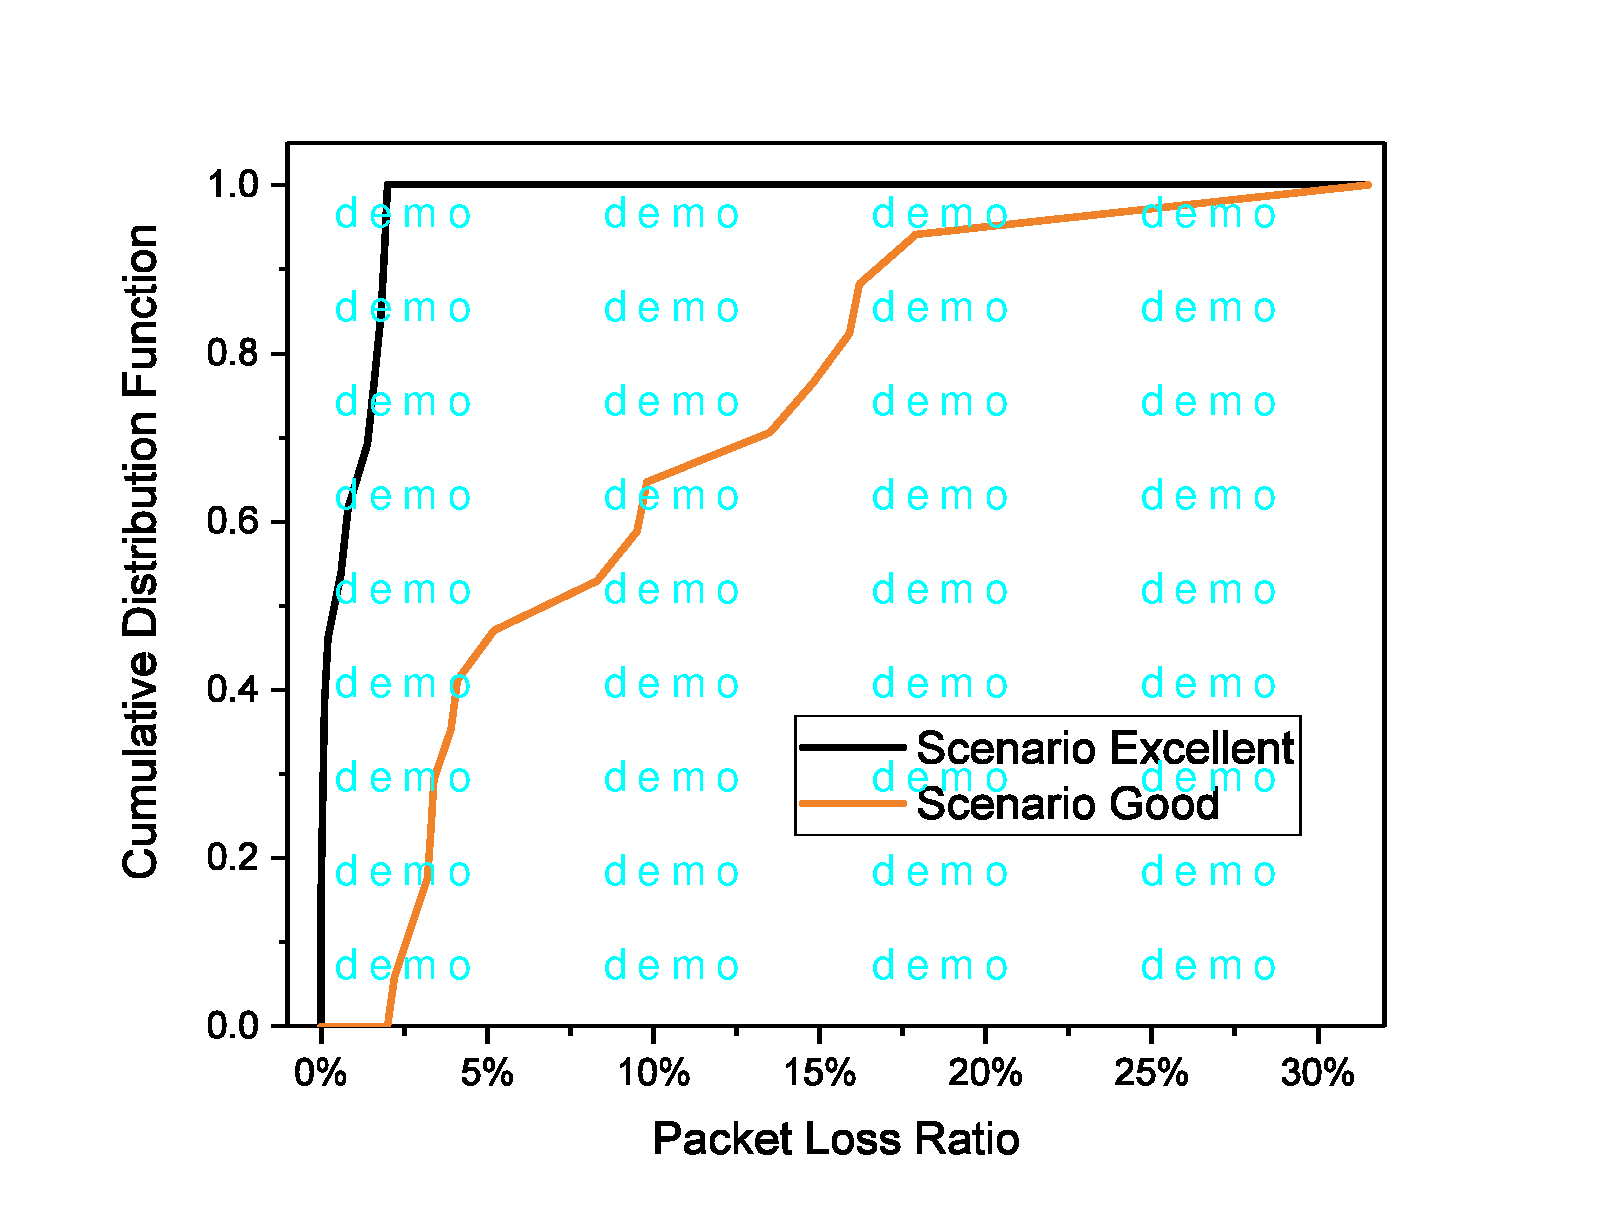
\includegraphics[width=0.7\textwidth]{chapters/chapter3/figures/capture-cdf-plr.pdf}
        \caption{两种场景平均丢包率的累积分布图}\label{fig:3:cdf-plr}
	\end{figure}
}

如图\nref{fig:3:cdf-plr},两种场景平均丢包率的累积分布出现偏离。Excellent场景的丢包率普遍较低,对时间隐通道的存在更敏感;Good场景中噪声干扰严重,丢包率上升,时间隐通道的检测难度增大。

\subsection{区间丢包数}
\label{chap:analyze:results:window}

\insertFigure{
	\begin{figure}[htbp]
		\centering
        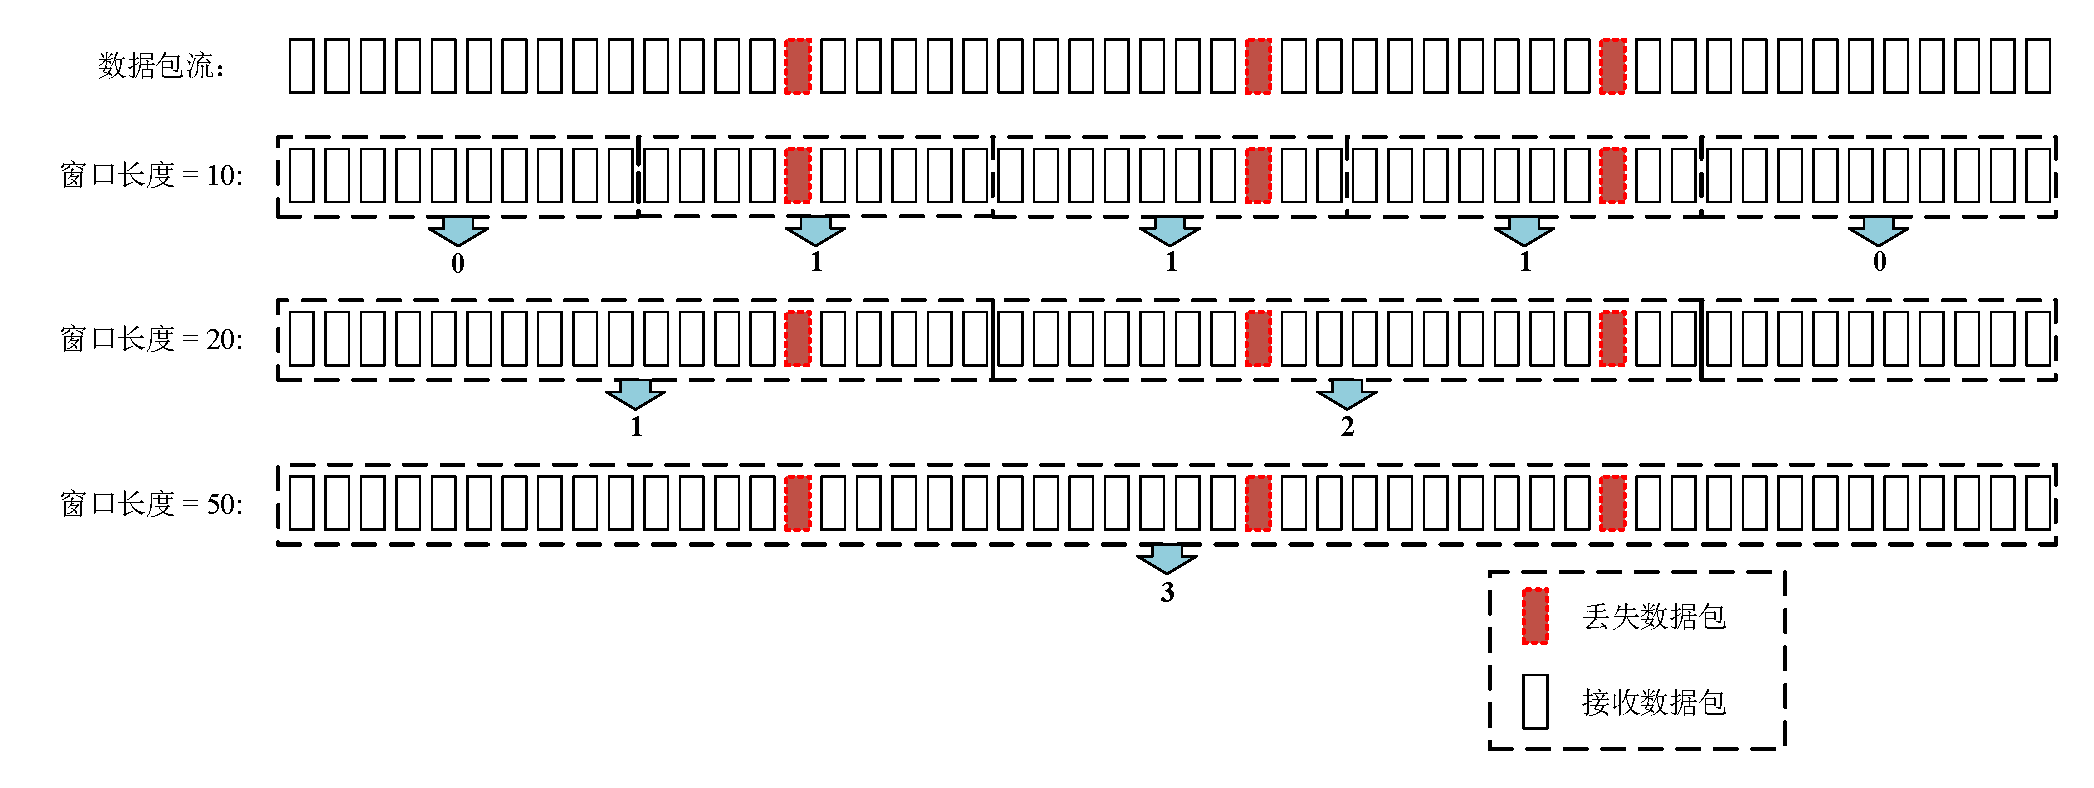
\includegraphics[width=0.99\textwidth]{chapters/chapter3/figures/win-size-count.pdf}
        \caption{区间长度与区间丢包数示意图}\label{fig:3:win-size-count}
    \end{figure}
}

%测试区间设定,以及不同场景下,各个区间的分布函数
如图\nref{fig:3:win-size-count},在相同丢包分布下,区间丢包数随着区间长度增大而累积。基于区间丢包数的检测方法,首先将数据包按照设定的区间长度划为独立区间,然后统计每个区间内的丢包数量。最终汇总各区间的统计结果,计算累积分布函数。

\insertFigure{
    \begin{figure}[htbp]
    \centering
        \subfigure[Excellent场景的累积分布函数]{
            \label{fig:3:capture:win-cdf:excellent}
            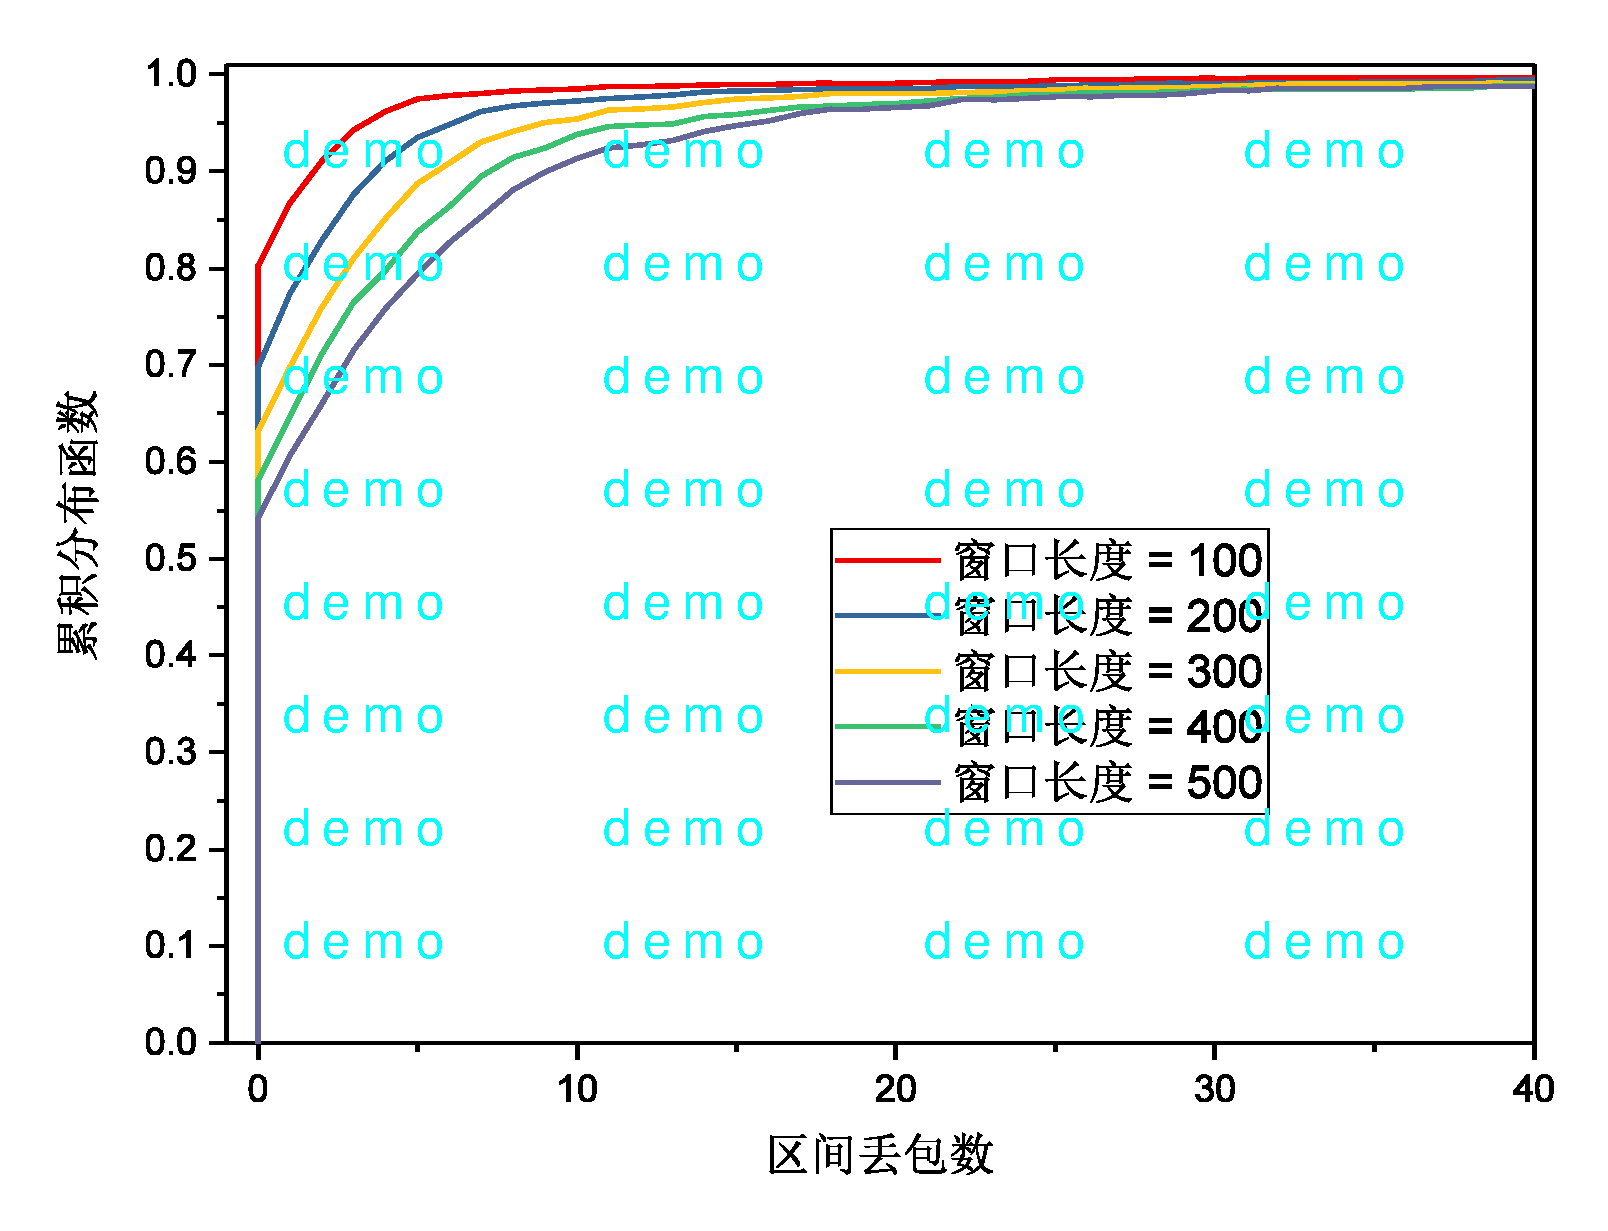
\includegraphics[width=0.48\textwidth]{chapters/chapter3/figures/capture-cdf-win-excellent.pdf}
        }
        \subfigure[Good场景的累积分布函数]{
            \label{fig:3:capture:win-cdf:good}
            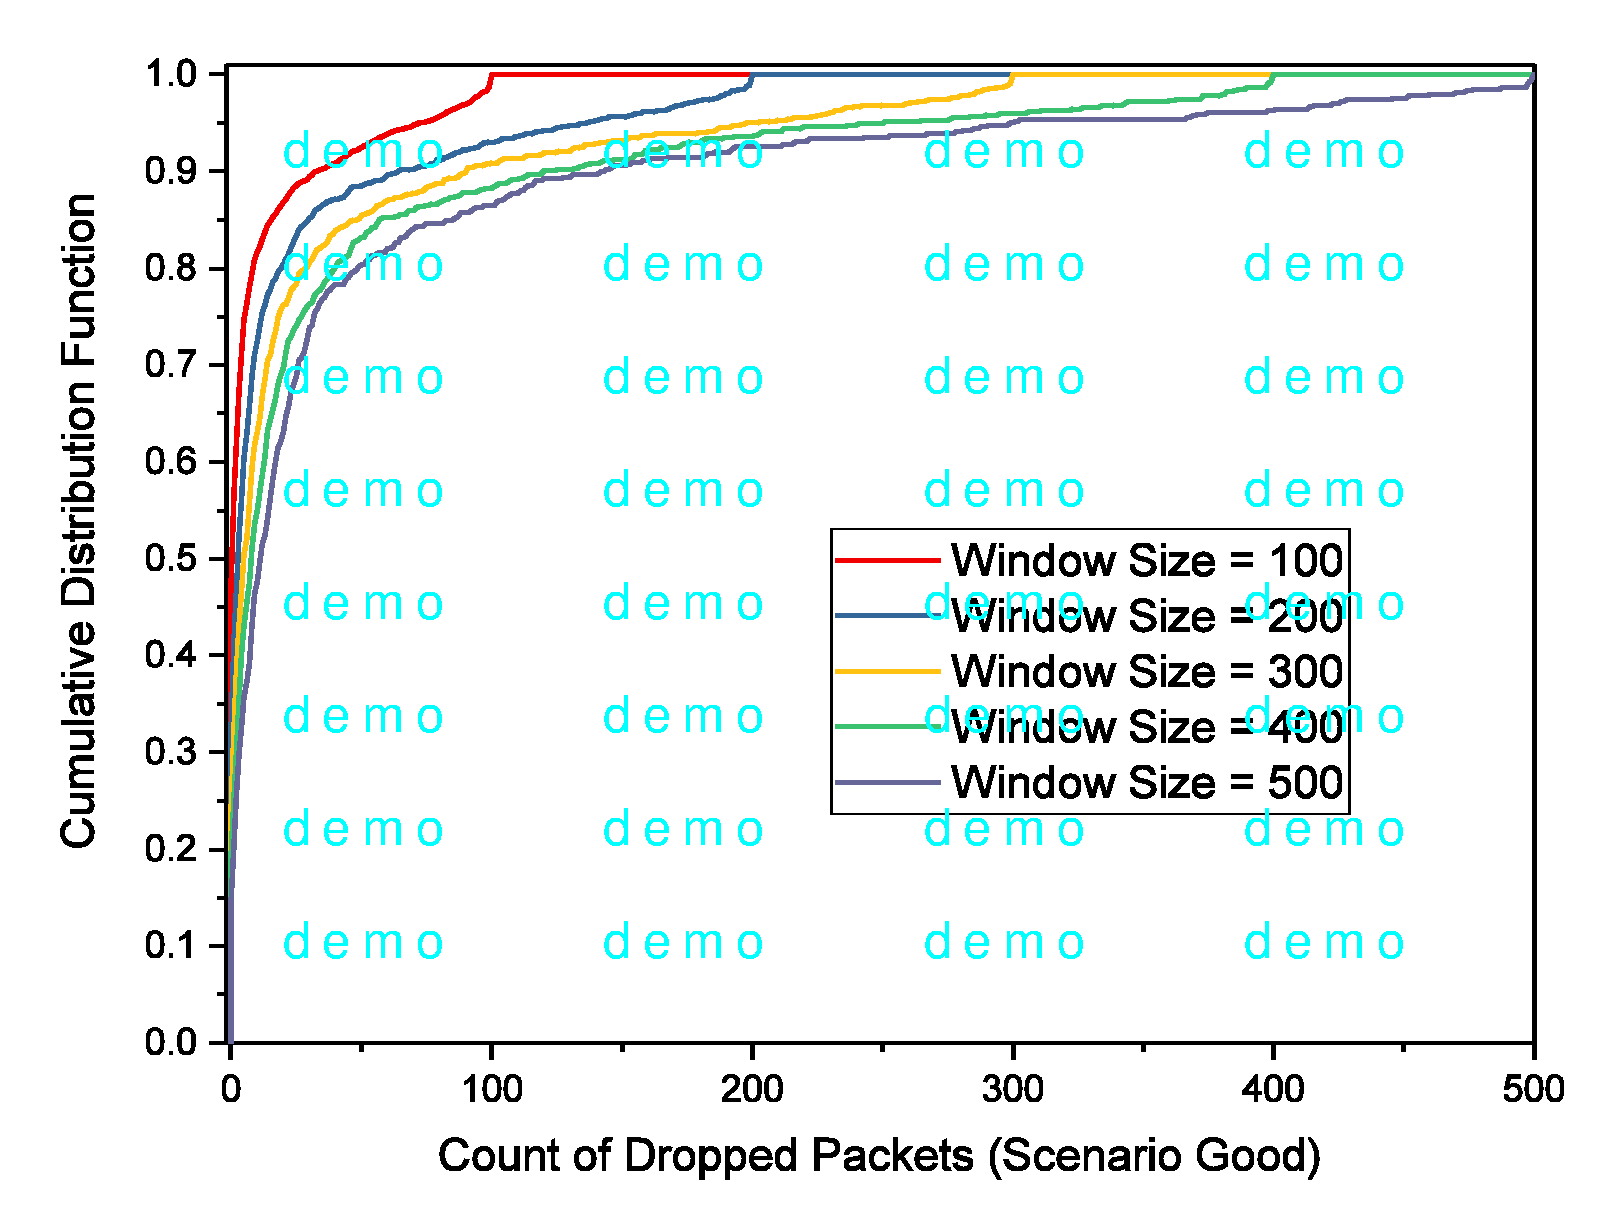
\includegraphics[width=0.48\textwidth]{chapters/chapter3/figures/capture-cdf-win-good.pdf}
        }
    \caption{区间丢包数的累积分布函数图}
    \label{fig:3:capture:win-cdf}
    \end{figure}
}

如图\nref{fig:3:capture:win-cdf},两种场景下的累积分布函数既存在相似性,又在存在局部差异。图\nref{fig:3:capture:win-cdf:excellent}中,丢包数量为$0$的区间均占据一半以上,并且CDF收敛到$1.0$的趋势较快,反应出网络质量较好。图\nref{fig:3:capture:win-cdf:good}中,曲线上升趋势与图\nref{fig:3:capture:win-cdf:excellent}类似,但丢包数量为$0$的部分比重较小,并且存在数据包全丢的区间。

\insertFigure{
    \begin{figure}[htbp]
        \centering
            \subfigure[区间长度为200时的概率质量函数]{
                \label{fig:3:capture:win-pmf:200}
                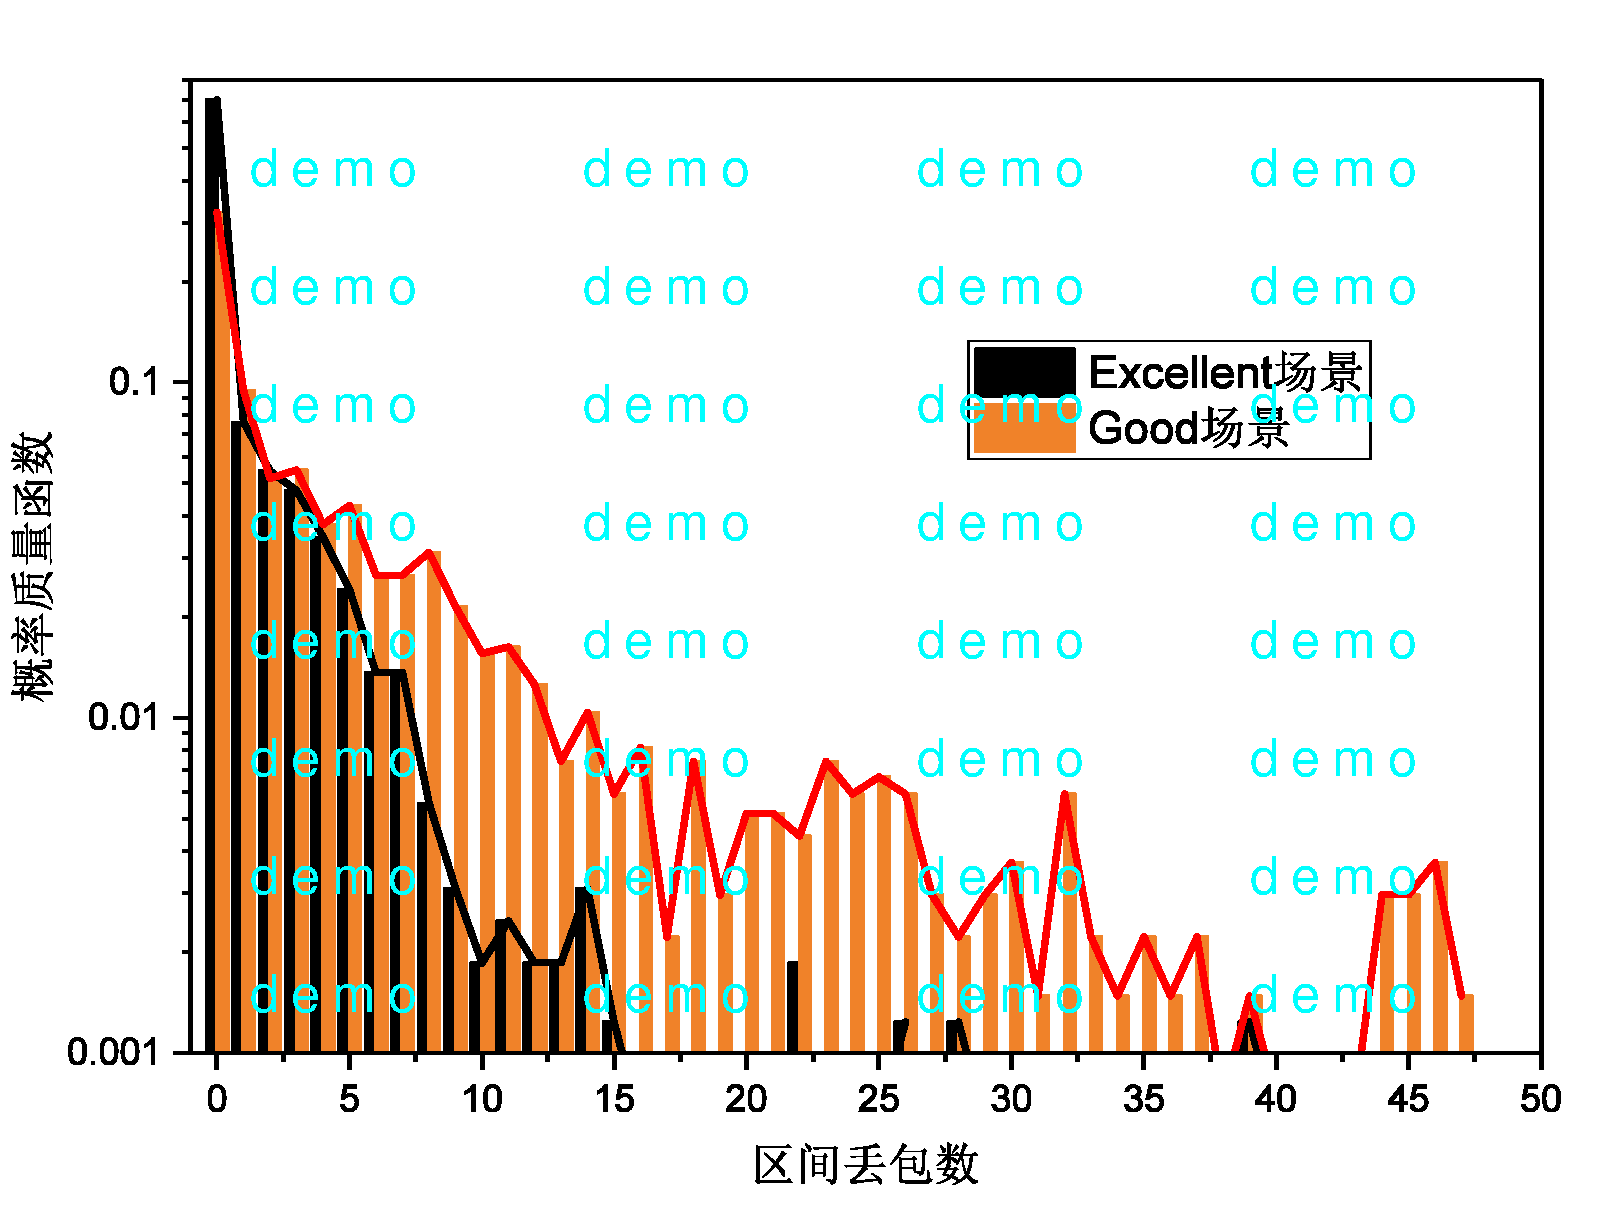
\includegraphics[width=0.48\textwidth]{chapters/chapter3/figures/capture-pmf-win200.pdf}
            }
            \subfigure[区间长度为400时的概率质量函数]{
                \label{fig:3:capture:win-pmf:400}
                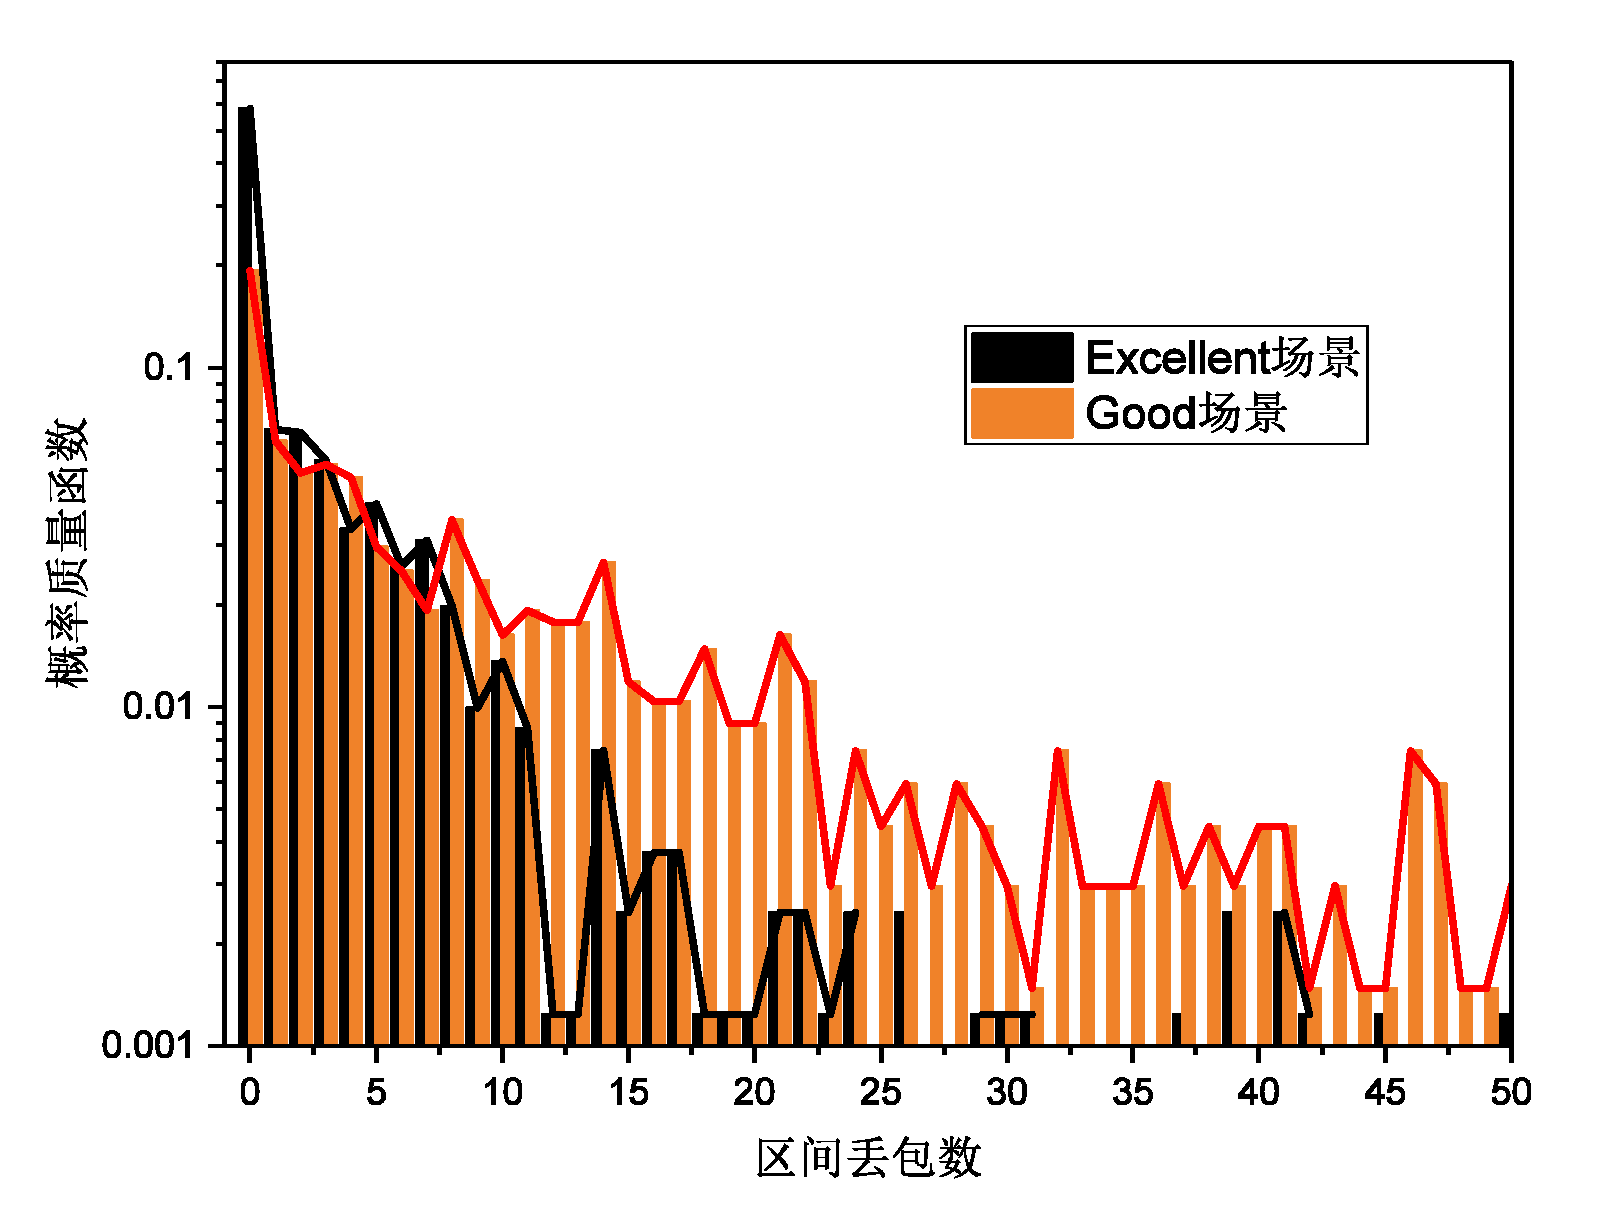
\includegraphics[width=0.48\textwidth]{chapters/chapter3/figures/capture-pmf-win400.pdf}
            }
        \caption{区间丢包数的概率质量函数图}
        \label{fig:3:capture:win-pmf}
        \end{figure}
}

如图\nref{fig:3:capture:win-pmf},概率质量函数在不同的场景中存在差异。概率质量函数存在不连续现象,并且不同场景中趋势差距较大,因此对区间丢包数的检验需要从整体的角度进行。

\subsection{数据包传输间隔}
\label{chap:analyze:results:ipd}

%IPD代表了什么
IPD是时间隐通道的基本测试对象,如图\nref{fig:2:cdf-ipd},发送与接收阶段的IPD分布存在差异。发送阶段存在两个聚集区间,而接收阶段曲线趋于平滑,证明网络缓冲及数据包转发削弱了原始IPD特征,导致接收方观测到的IPD接近正偏态分布。

%两种场景下抓包得到的IPD分布
\insertFigure{
    \begin{figure}[htbp]
    \centering
        \subfigure[IPD分布的累积分布函数图]{
            \label{fig:3:capture:ipd:cdf}
            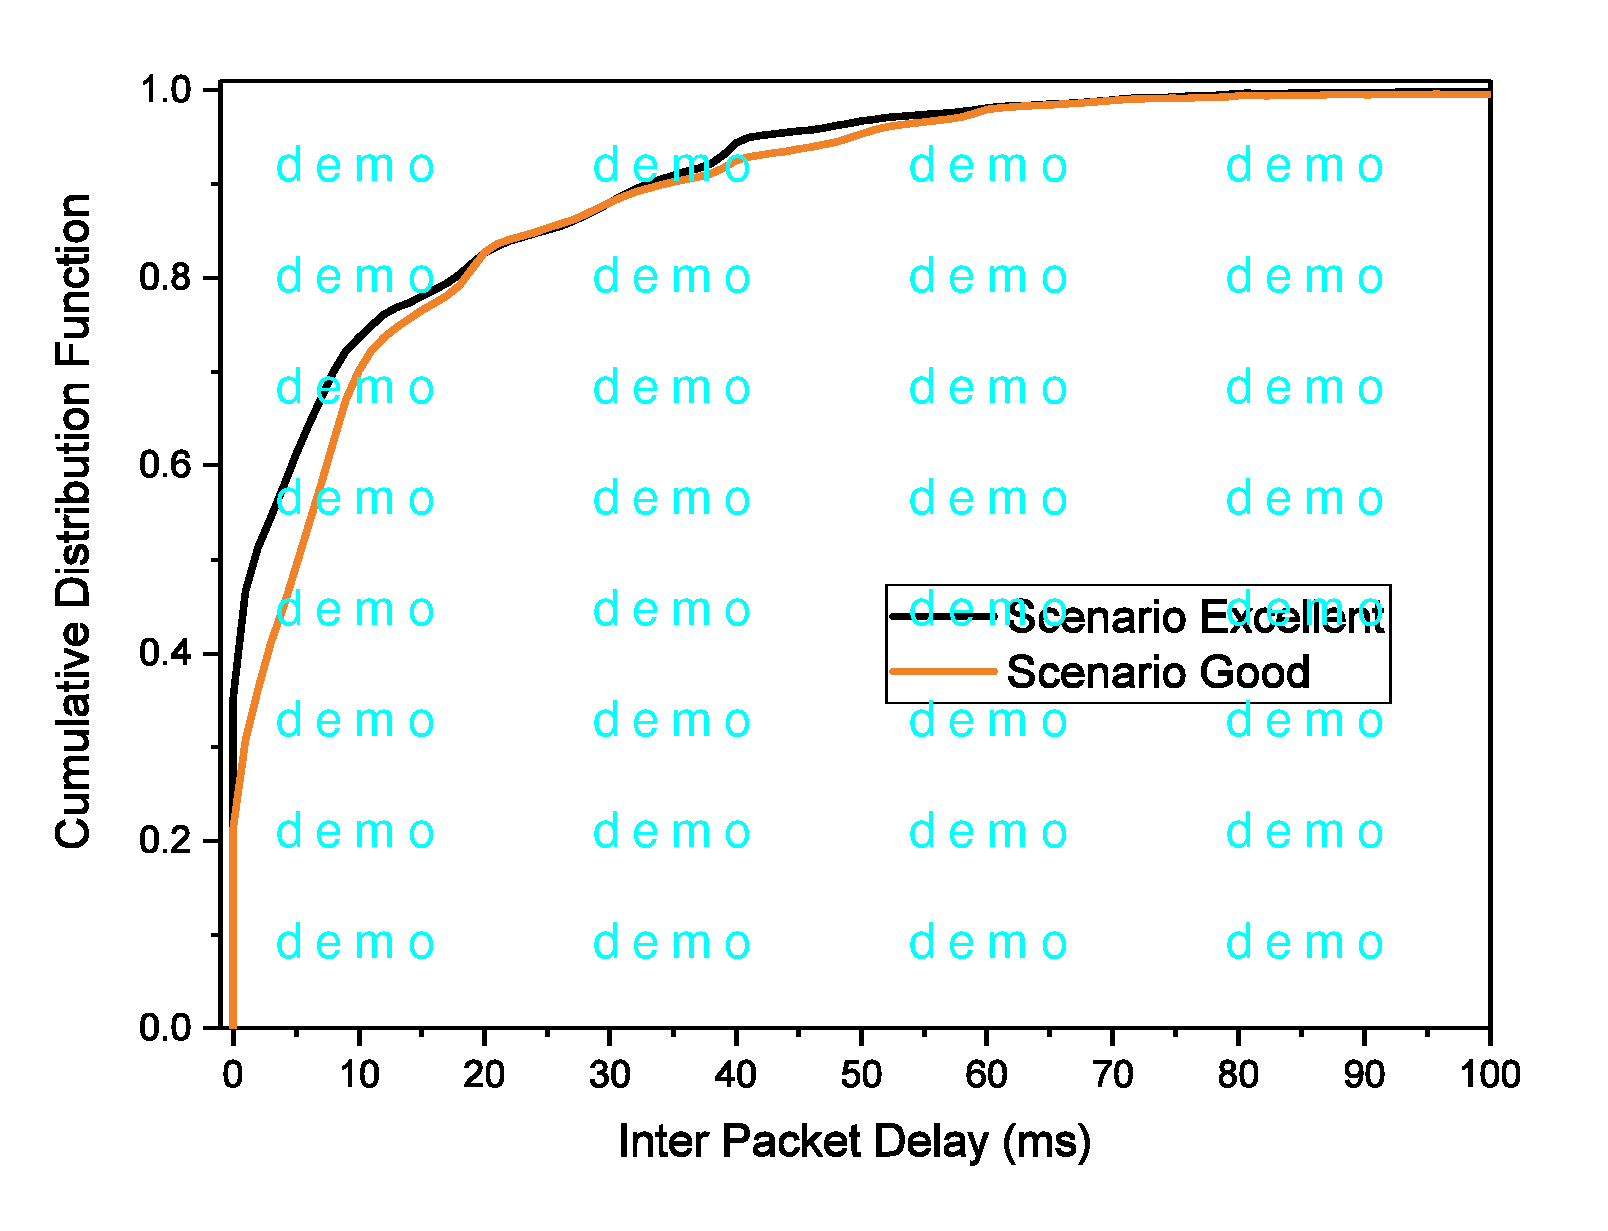
\includegraphics[width=0.48\textwidth]{chapters/chapter3/figures/capture-ipd-cdf.pdf}
        }
        \subfigure[IPD分布的概率质量函数图]{
            \label{fig:3:capture:ipd:pmf}
            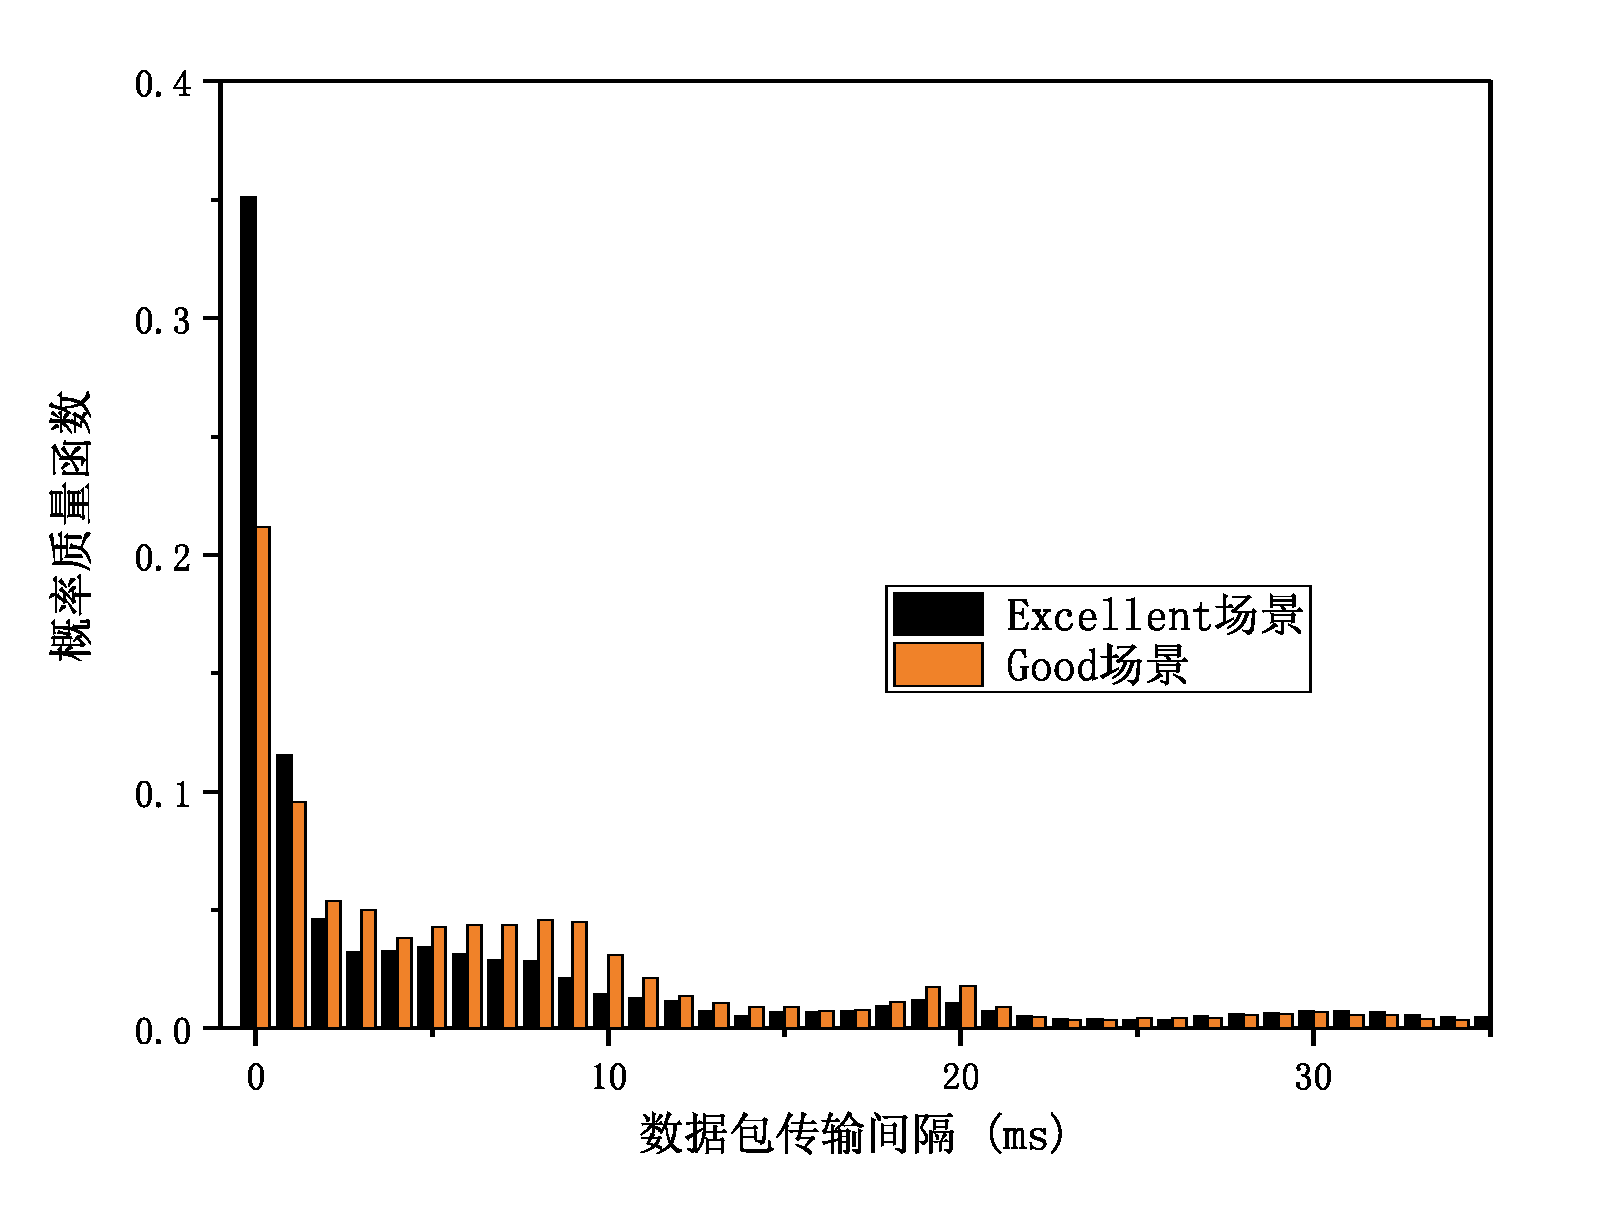
\includegraphics[width=0.48\textwidth]{chapters/chapter3/figures/capture-ipd-pmf.pdf}
        }
    \caption{VoLTE视频数据包IPD分布图}
    \label{fig:3:capture:ipd}
    \end{figure}
}

图\nref{fig:3:capture:ipd}中,分别展示了两种场景下的IPD分布情况。如图\nref{fig:3:capture:ipd:cdf},两种场景中的趋势及数值范围均近似,证明丢包事件对IPD分布的影响较小。图\nref{fig:3:capture:ipd:pmf}中,IPD的概率质量函数在不同场景中也具有近似的趋势。综合概率质量函数及累积分布函数的变化趋势,对于基于主动丢包的时间隐通道,仅通过IPD分布进行检测是不完善的。另一方面,证明了基于主动丢包的时间隐通道构建方法,在当前检测方法面前具有较好的隐蔽性。

\subsection{连续丢包}
\label{chap:analyze:results:burst}

%什么是连续丢包数
网络中的丢包事件,通常分为随机丢包和一定长度的连续丢包,随机丢包为随机丢失的单个数据包,连续丢包为连续丢失的多个数据包。\nupcite{816237,6711984}。对于视频通话,随机丢包持续影响视频质量,连续丢包主要影响通话稳定性。\nupcite{5977359,6894614,1709847}本文中,将随机丢包作为连续丢包的一种特殊情况,即长度为1的连续丢包,在分布统计中统一处理。

%两种场景下,测试得到的连续丢包数信息
\insertFigure{
    \begin{figure}[htbp]
        \centering
            \subfigure[连续丢包数的累积分布函数图]{
                \label{fig:3:capture:burst:cdf}
                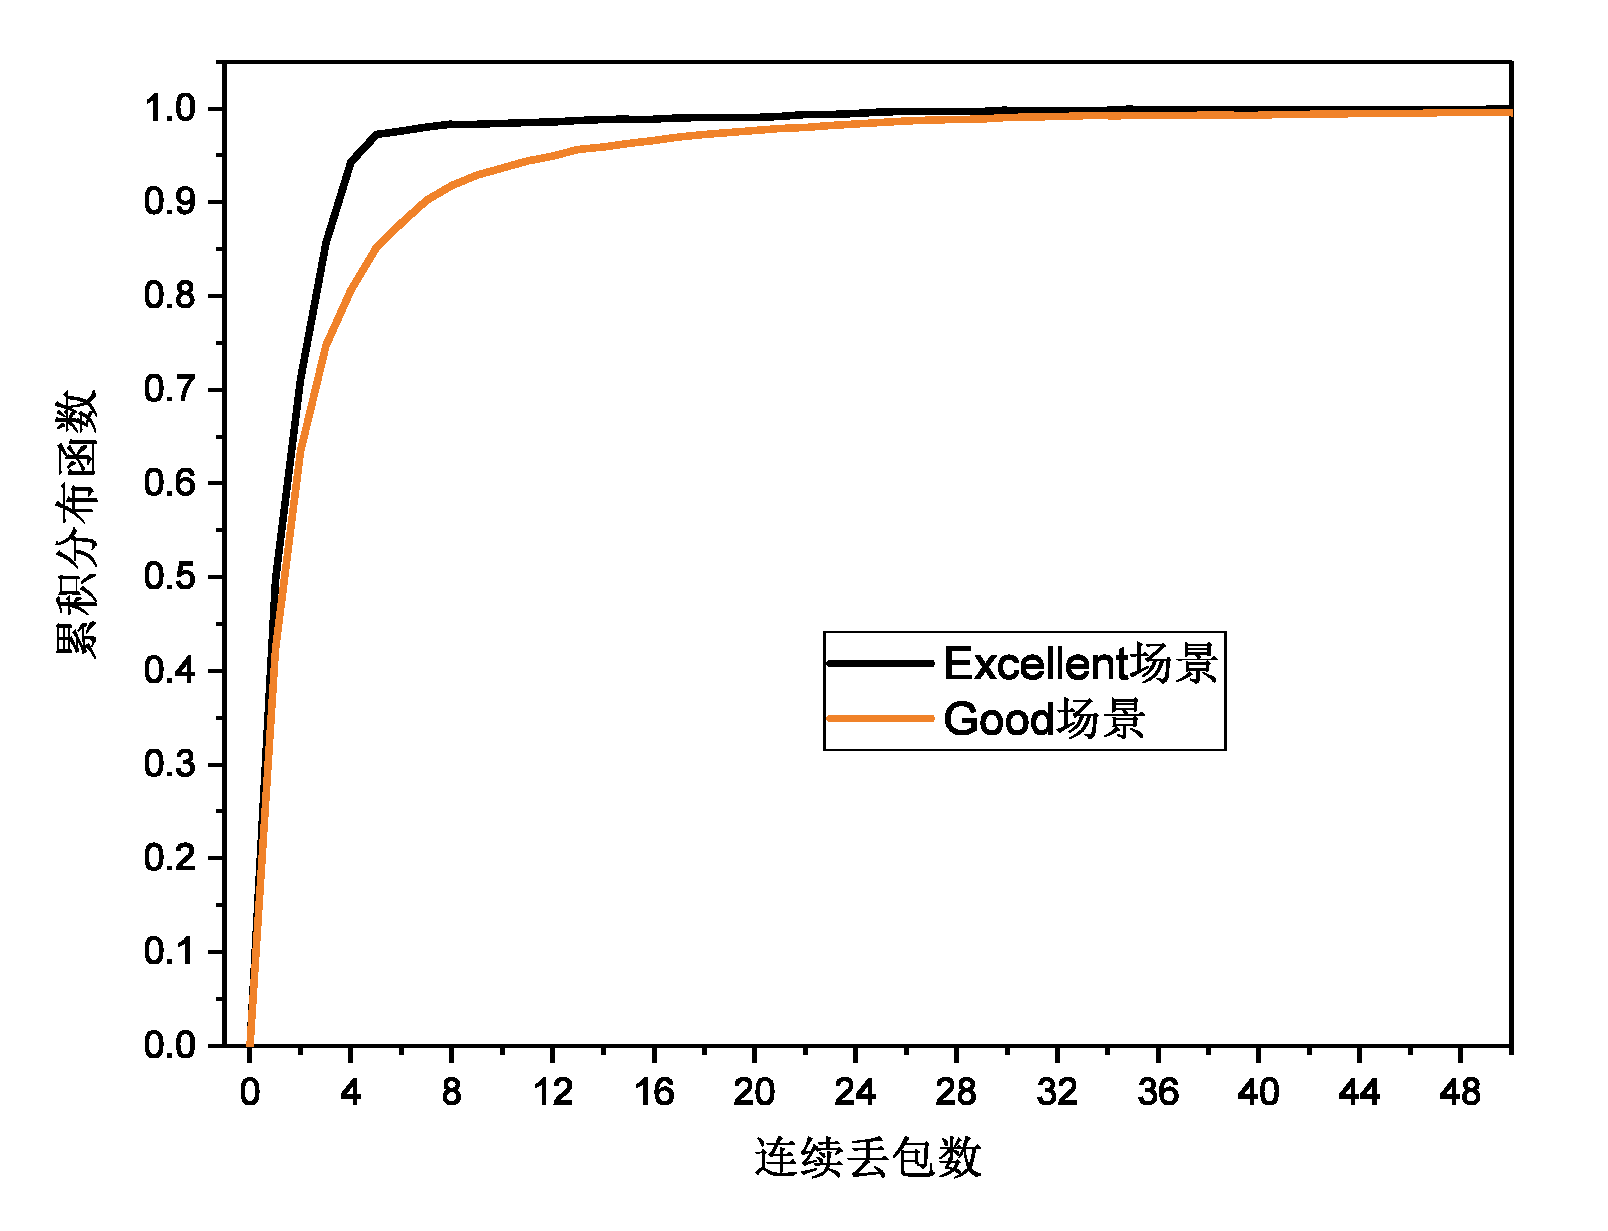
\includegraphics[width=0.48\textwidth]{chapters/chapter3/figures/capture-cdf-burst.pdf}
            }
            \subfigure[连续丢包数的概率质量函数图]{
                \label{fig:3:capture:burst:pmf}
                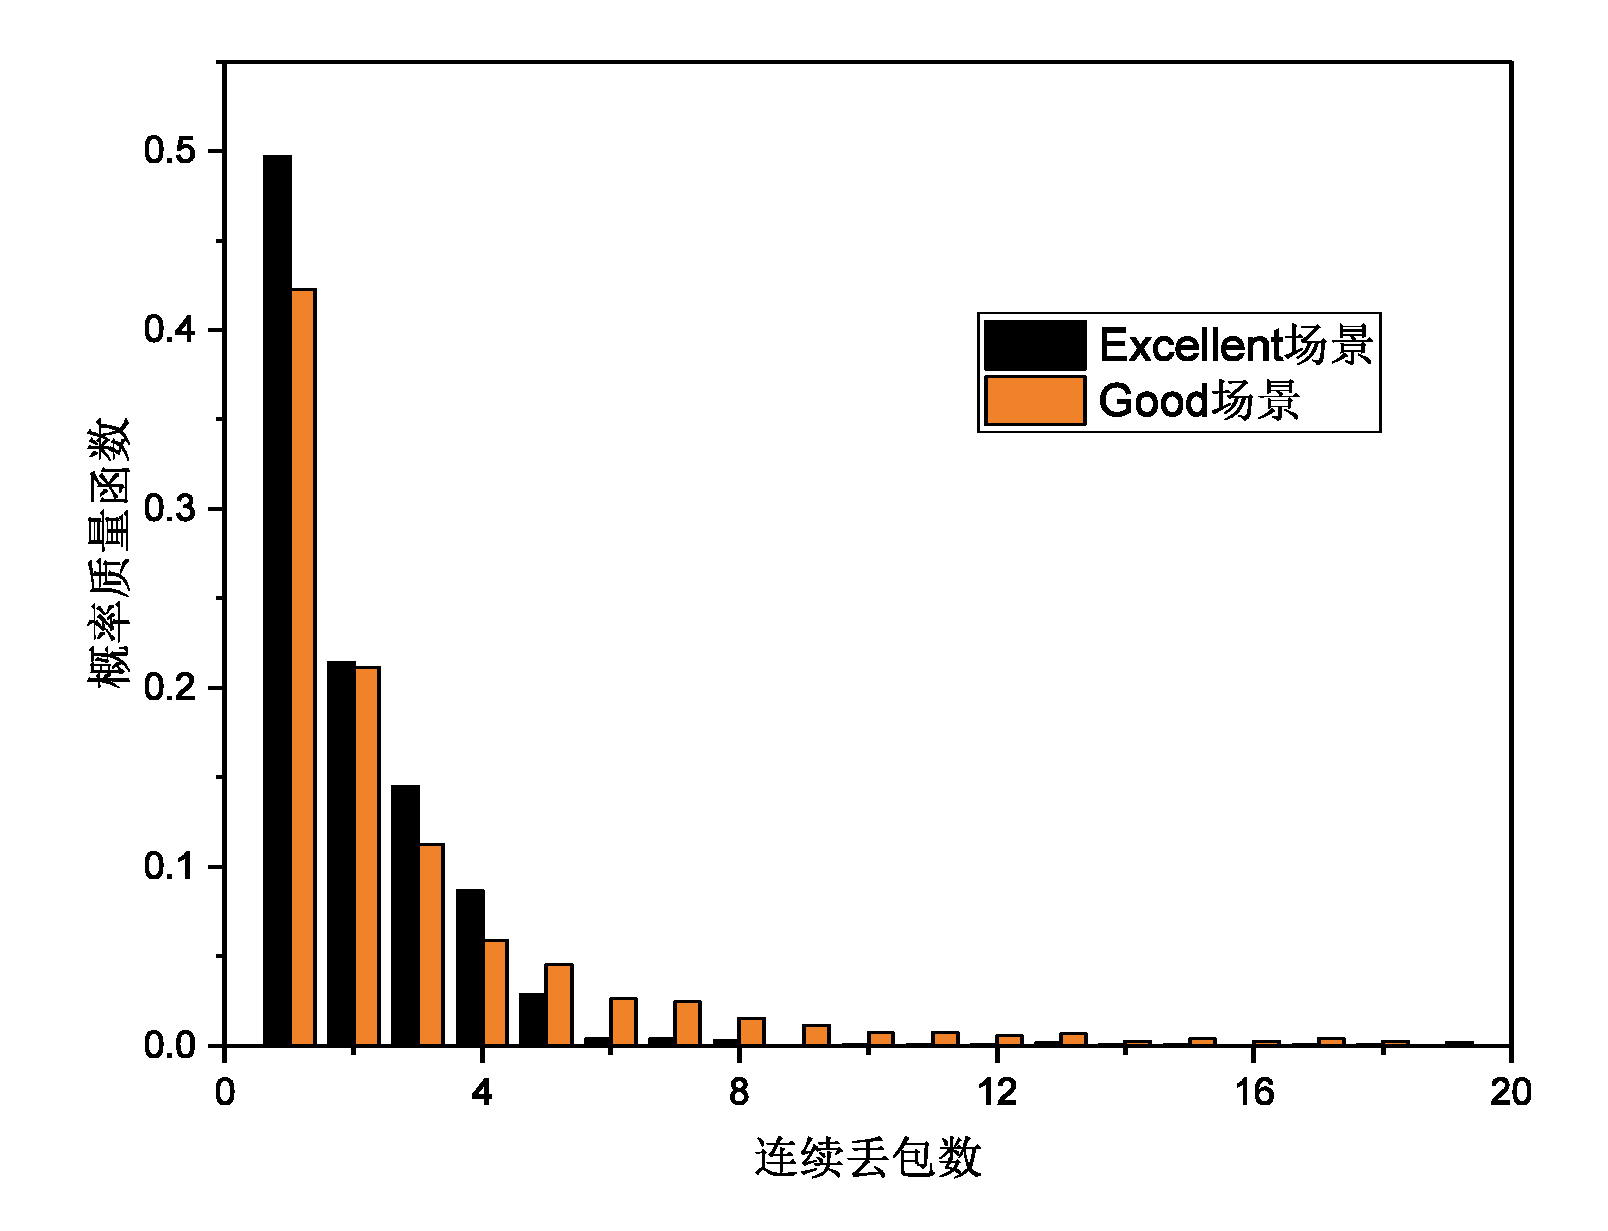
\includegraphics[width=0.48\textwidth]{chapters/chapter3/figures/capture-pmf-burst.pdf}
            }
        \caption{两种场景中连续丢包数的分布图}
        \label{fig:3:capture:burst}
    \end{figure}
}

如图\nref{fig:3:capture:burst},在两种网络场景中,连续丢包数的分布趋势趋于一致。具体到局部特征,Excellent场景与Good场景在连续丢包数大于1的部分,在总体中的占比存在差异。如图\nref{fig:3:capture:burst:cdf},Excellent场景中,连续丢包数普遍较小,累积分布函数曲线在起始阶段上升迅速;Good场景中,连续丢包导致CDF曲线趋近1的速度减缓。如图\nref{fig:3:capture:burst:pmf},连续丢包数的概率质量函数具有规律,并且分布曲线平滑连续,满足检测要求。基于主动丢包的时间隐通道,导致长度为1的连续丢包数增多,对分布曲线的趋势及数值存在影响。